\documentclass[a4paper,10pt]{article}
\usepackage[utf8x]{inputenc}
%\usepackage[utf8]{inputenc}
\usepackage{graphicx}
\usepackage{color}
\usepackage[table]{xcolor}
\usepackage{url}
\usepackage{enumitem}% http://ctan.org/pkg/enumitem
%\usepackage{algorithm, algorithmicx}
\usepackage[noend]{algpseudocode}
\usepackage{comment}
\usepackage[standard]{ntheorem}
\usepackage{multirow}
\usepackage{subcaption}
\usepackage{caption}
\usepackage[noadjust]{cite}
\usepackage{pdflscape}
\usepackage{lipsum}
\usepackage{capt-of}
\usepackage[linesnumbered,ruled,vlined]{algorithm2e}
\usepackage{amsmath,amssymb,amsfonts}
\usepackage{threeparttable}
\usepackage{booktabs}
\newtheorem{notation}{Notation}


\setlength{\textheight}{9.2in}
\setlength{\textwidth}{6.4in}

\setlength{\oddsidemargin}{0mm}
\setlength{\evensidemargin}{0mm}
\setlength{\topmargin}{-0.3in}

\newcommand{\sat}{$\;\triangleleft\;$}
\newcommand{\nsat}{$\;\ntriangleleft\;$}

\newcommand{\subgraphname}{part}
\newcommand{\subgraphnamespace}{part }
\newcommand{\subgraphnameCaps}{Part}

\usepackage[bookmarks=false]{hyperref}
\hypersetup{
	colorlinks,
	citecolor=black,
	filecolor=black,
	linkcolor=black,
	urlcolor=black
}
\graphicspath{{./images/}{./lstmResults/}{./cnnResults/}{./somResults}}

\newcommand{\numBytesOffChip}{\mathbb{B}}
\newcommand{\numOverlap}{\delta}
\newcommand{\busWidth}{BW}
\newcommand{\dataWidth}{DW}
\newcommand{\dataLength}{l}
\newcommand{\addressSym}{Addr}
\newcommand{\BuffSize}{buffSize}
%\newcommand{\EXPANDER}{{\scriptsize  {EXPANDER}}\xspace}

\begin{document}
	
\begin{titlepage}
	
	\begin{center}
		
		\vspace{4cm}
		\LARGE \textbf{A FRAMEWORK FOR MAPPING NEURAL NETWORKS ON PARALLEL ARCHITECTURES}\\
		
		\vspace{2cm}
		
		\large {A synopsis submitted in partial fulfillment of the requirements for the degree\ \\}
		\vspace{0.5cm}
		\large {of\ \\}
		\vspace{0.5cm}
		\Large \textbf{Doctor of Philosophy \ \\}
		\vspace{0.5cm}
		
		\large \ \\ \ \\ Submitted by: \ \\
		\Large \textbf{SAURABH TEWARI \ \\ (2015CSZ8046)} 
		
		\large {\ \\ under the guidance of \ \\}
		% \vspace{0.2cm}
		\large \textbf{ Prof. Anshul Kumar\\ }
		\large \textbf{ Prof. Kolin Paul\\ }
		% \large {Department of Computer Science and Engineering \ \\}
		\vspace{2.0cm}
		\hspace{0cm}
		
\includegraphics[scale=1.0]{images/logo.pdf} \\
		\vspace{2.0cm} 
		\Large {DEPARTMENT OF COMPUTER SCIENCE \& ENGINEERING}\\
		\Large {INDIAN INSTITUTE OF TECHNOLOGY DELHI \\ NEW DELHI}\\
		% \vspace{2cm}
	\end{center}
	
\end{titlepage}
\pagenumbering{roman}
\section*{List of Included Papers}
This thesis is based on the following publications:

\textbf{Published:}

\newcounter{saveenum}

\begin{enumerate}
\item \textbf{S. Tewari}, A. Kumar and K. Paul, ``\textit{SACC: Split and Combine Approach to Reduce the Off-chip Memory Accesses of LSTM Accelerators}'', in DATE 2021.

\item \textbf{S. Tewari}, A. Kumar and K. Paul, ``\textit{Minimizing Off-Chip Memory Access for CNN Accelerators}'', in IEEE Consumer Electronics Magazine 2021.

\item \textbf{S. Tewari}, A. Kumar and K. Paul, ``\textit{Bus Width Aware Off-Chip Memory Access Minimization for CNN Accelerators}", in ISVLSI 2020.

\item D. Stathis, Y. Yang, \textbf{S. Tewari}, A. Hemani, K. Paul, M. Grabherr and R. Ahmad, ``\textit{Approximate Computing Applied to Bacterial Genome Identification using Self-Organizing Maps}'', in ISVLSI 2019.

\setcounter{saveenum}{\value{enumi}}
\end{enumerate}



%\textbf{In-review/Under preparation:}
%\begin{enumerate}
%  \setcounter{enumi}{\value{saveenum}}
%
%\item \textbf{Rajesh Kedia}, Shikha Goel, M. Balakrishnan, Kolin Paul, and Rijurekha Sen. ``\textit{Design space exploration of FPGA based system with heterogeneous DNN accelerators}''. Submitted to IEEE Embedded Systems Letters.
%
%\item \textbf{Rajesh Kedia}, M. Balakrishnan, and Kolin Paul. ``\textit{An integrated flow for designing Context-aware Adaptive Embedded Systems}'' -- under preparation.
%
%\item Shikha Goel, \textbf{Rajesh Kedia}, M. Balakrishnan, and Rijurekha Sen. ``\textit{INFER: INterFerence-aware Estimation of Runtime for concurrent DNN execution on DPUs}'' -- under preparation.
%
%\end{enumerate}




\newpage
\setcounter{tocdepth}{2}
\tableofcontents
\newpage

\pagenumbering{arabic}
\begin{comment}
	1. Introduction - 2 pages
	2. Related work - 0.5 pages
	3. Overall flow - 0.75 pages
	4. Graphical representation - 2 pages
	5. DSE flow - 2 pages
	6. Runtime controller generation - 1.5 page
	7. Case studies - 3.5 pages
	a. RBD - (0.5 page)
	b. MAVI - (2 pages)
	c. DPU - (1 page)
	8. Conclusion - 0.5 page
	9. References - 2 pages
\end{comment}
\section{Introduction}
Deep neural networks (DNNs) are machine learning algorithms used in wide range of applications due to their high accuracy. To improve the accuracy, recent DNNs use large number of parameters and perform memory and compute intensive operations. 
DNNs have training and inference phase. They are first trained (training phase) to determine the learning parameters (weights and biases) and then these learned parameters are used in applications to predict the output (inference phase). The training of these deep networks require large number of inputs and several iterations to update the weights and baises. This may take several hours to days and require significant computations. The training is mostly performed offline on high end machines and servers. The parameters learned during training phase are then used in applications for inference. In this work, we focus on the inference phase of DNNs, which is performed energy constraint devices.

Many latest consumer electronics devices like smartphones and home appliances use DNNs to provide new features and improve user experiences. The manufacturers are shifting the processing of these algorithms to edge devices to improve response time and eliminate network bandwidth issues. These edge devices, usually battery operated, commonly use DNN accelerators to speed-up processing and reduce energy consumption. 

Deep neural networks consists of an input layer, an output layer and several intermediate hidden layers. Recent DNN can have upto thousands of hidden layers. Figure~\ref{fig:typesNN} shows two broad class of neural networks. Most of the recent DNNs can be classified as following,
\begin{enumerate}
	\item Feed forward: This class of NNs use the outputs from a layer as input to the subsequent layers. For a given input, output is independent of previous seen inputs. Convolution Neural Networks (CNN) belongs to this category and commonly used for image and video processing applications. 
	\item Recurrent NN: This class of NNs maintain the state information to store the contextual information and state is updated with every input. The output depends on the input as well as the state information. For the same input, the output may vary depending on the current state. This class of networks is used for processing sequential data e.g. speech recognition and language processing tasks. Long Short Term Memory networks (LSTMs) are one of the most popular variants of RNN.
\end{enumerate}
\begin{figure}[!htb]
	\centering
	\subfloat[Feed Forward NN]
	{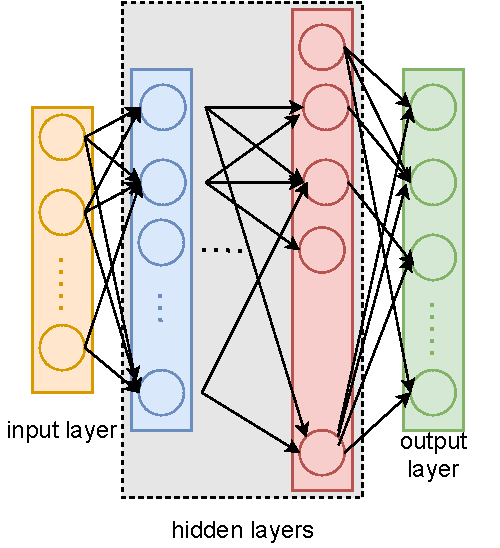
\includegraphics[width=0.25\textwidth]{feedForwardNN.pdf}
		\label{fig:feedForwardNN}}
	\hfil
	\subfloat[Recurrent NN]
	{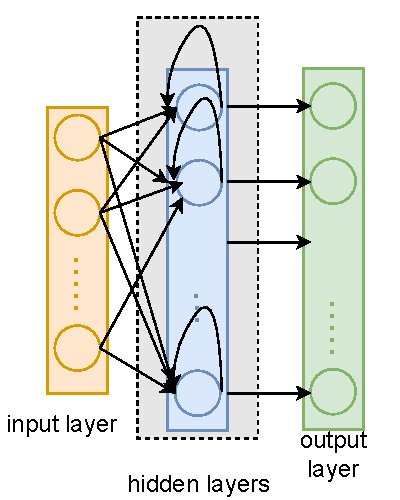
\includegraphics[width=.25\textwidth]{recurrentNN.pdf}
		\label{fig:recurrentNN}}
	\caption{Feedforward and Recurrent Neural Networks.}
	\label{fig:typesNN}
	\vspace{-1.0em}	
\end{figure}
To improve the performance  FPGA~\cite{zhang2015optimizing,wei2019overcoming,gokhale2014240,8742284,gupta2015deep,alwani2016fused}, GPU~\cite{chetlur2014cudnn} and ASIC~\cite{Chen2016EyerissAS,chen2014diannao,chen2014dadiannao,du2015shidiannao} accelerators with large number of parallel compute resources are proposed. While these accelerators can match the performance to some extent, their energy efficiency is still a concern.  Energy efficiency of DNN accelerators is of paramount importance for their ubiquitous usage in energy constrained devices like smart-phones, tablets etc. More than 80\% of the overall energy consumption of these accelerators is due to off-chip memory accesses~\cite{chen2014diannao}. 
%Figure~\ref{fig:dnnAccelerator} shows a typical DNN accelerator system, which consists of an accelerator chip and off-chip memory. The accelerator chip has small on-chip buffer and an array of processing elements (PE) to perform parallel computations. 
%\begin{figure}[!htb]
%	\centering
%	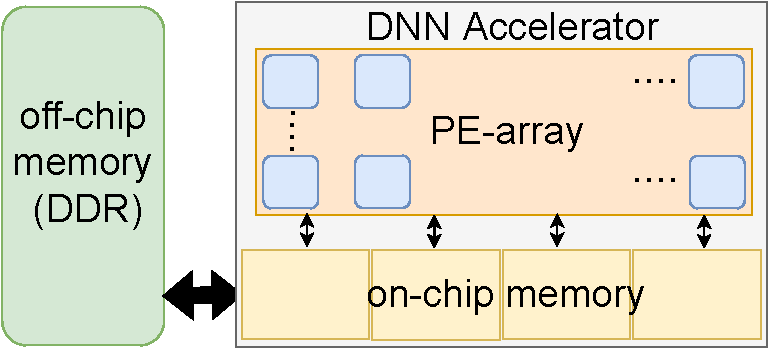
\includegraphics[width=0.4\linewidth]{DNNAccelerator}
%	\caption{A typical DNN accelerator architecture}
%	\label{fig:dnnAccelerator}
%\end{figure}
In this work, we propose approaches to optimize the performance and energy efficiency of feed forward and recurrent neural network accelerators during inference phase.

\subsection{Impact of off-chip memory access}
\subsubsection{Performance}
DNN accelerators have large number of processing elements (PEs) to exploit the parallelism of DNNs. While these PEs can perform several operations per cycle, their performance is limited by off-chip memory bandwidth. In the near forseeable future, off-chip memory accesses limits the system performance~\cite{williams2009roofline}. Fig.~\ref{fig:roofline} shows, two kernels with different compute intensity (FLOPS/byte), possibly due to different data reuse techniques. Kernel 2 can perform more computations per byte, compared to Kernel 1. Performance of Kernel 2 is limited by computational roof and it utilizes the compute resources fully (compute bound), while Kernel 1's performance is limited by memory bandwidth (memory bound).
\begin{figure}[!htb]
	\centering
	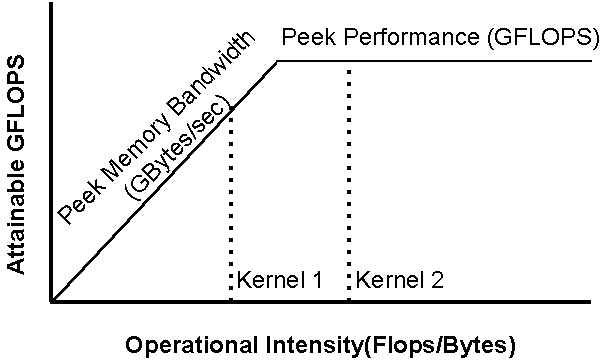
\includegraphics[width=0.5\linewidth]{roofline}
	\caption{roofline model}
	\label{fig:roofline}
\end{figure}
Memory bound kernels results in under-utilization of compute resources, which results in degraded performance and energy consumption. To improve the DNN accelerators' performance, maximizing the data reuse from on-chip memories is essential.
\subsubsection{Energy efficiency}
The energy of DNN accelerators is the sum of computations and data accesses energy. 
\begin{equation}
	E=E_{comp} + E_{data}
\end{equation}
where $E_{comp}$ and $E_{data}$ are the computation and data movement energy, respectively. $E_{comp}$ for a DNN layer depends on the number of operations in the layer, which is fixed as it depends on layer shape e.g. number of activations, filters, and filter sizes. However $E_{data}$ can be optimized using data reuse techniques. Typically DNN accelerator system has multiple levels of memory hierarchy. Memories at different levels of hierarchy have different sizes, access-energies and access-time. The off-chip memory (DDR), at the top of the hierarchy, has the largest capacity, and highest access-energy and access-time compared to memories at lower level of hierarchy.  The off-chip memory access energy is upto two orders higher compared to on-chip memory access energy. 

Figure~\ref{fig:dataAccessEnergy} illustrates the impact of data reuse on the energy efficiency of a system with 2 levels of memory (DDR and L1). The energy efficiency can be expressed as below,
\begin{figure}[!htb]
	\centering
	\subfloat[no data reuse]
	{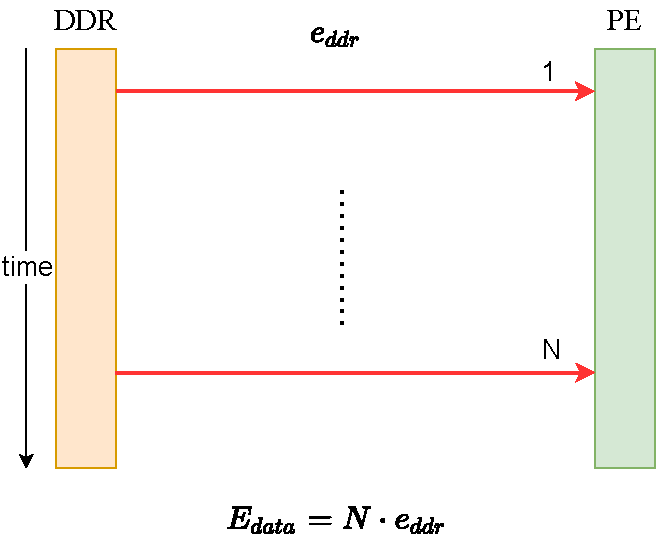
\includegraphics[width=0.3\textwidth]{energyDDR_noreuse.pdf}
		\label{fig:energyNoReuse}}
	\hfil
	\subfloat[with reuse ($\times{n}$) from L1]
	{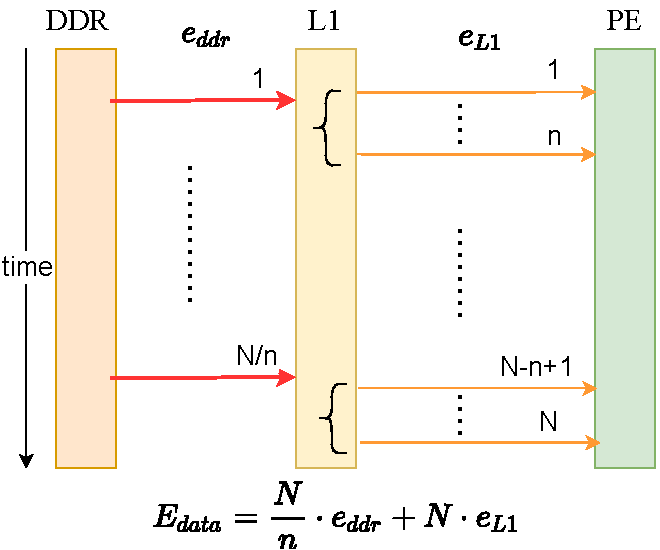
\includegraphics[width=.3\textwidth]{energy_reuse.pdf}
		\label{fig:energy_reuse}}
	\caption{Data access energy $E_{data}$.}
	\label{fig:dataAccessEnergy}
	\vspace{-1.0em}	
\end{figure}
\begin{align*}
	\text{Energy-efficiency} &= (1-\frac{E^2_{data}}{E^1_{data}})\times{100}\\
	&= (1-(\frac{1}{n}+\frac{e_{L1}}{e_{ddr}}))\times{100}
\end{align*}
As, $e_{L1} << e_{DDR}$, the ratio $\frac{e_{L1}}{e_{ddr}}$ is very small, the energy efficiency depends on number of reuses ($n$) from on-chip memory $L1$. It improves considerably with increasing the number of data reuse ($n$). 

Reducing the off-chip memory accesses is the key to reduce the energy consumption of DNN accelerators. State of the art DNN accelerators aim to maximize the data reuse from on-chip memory to reduce the off-chip memory accesses. Our work aims to improve the performance and energy efficiency of DNN accelerators by reducing the off-chip memory accesses and maximizing the data reuse from on-chip memories.
\section{Mapping Framework}
Towards this end we propose a mapping framework which optimizes the off-chip memory accesses for feed-forward and recurrent neural networks. Our main contributions in this thesis dessertations are
\begin{figure}[ht]
	\centering
	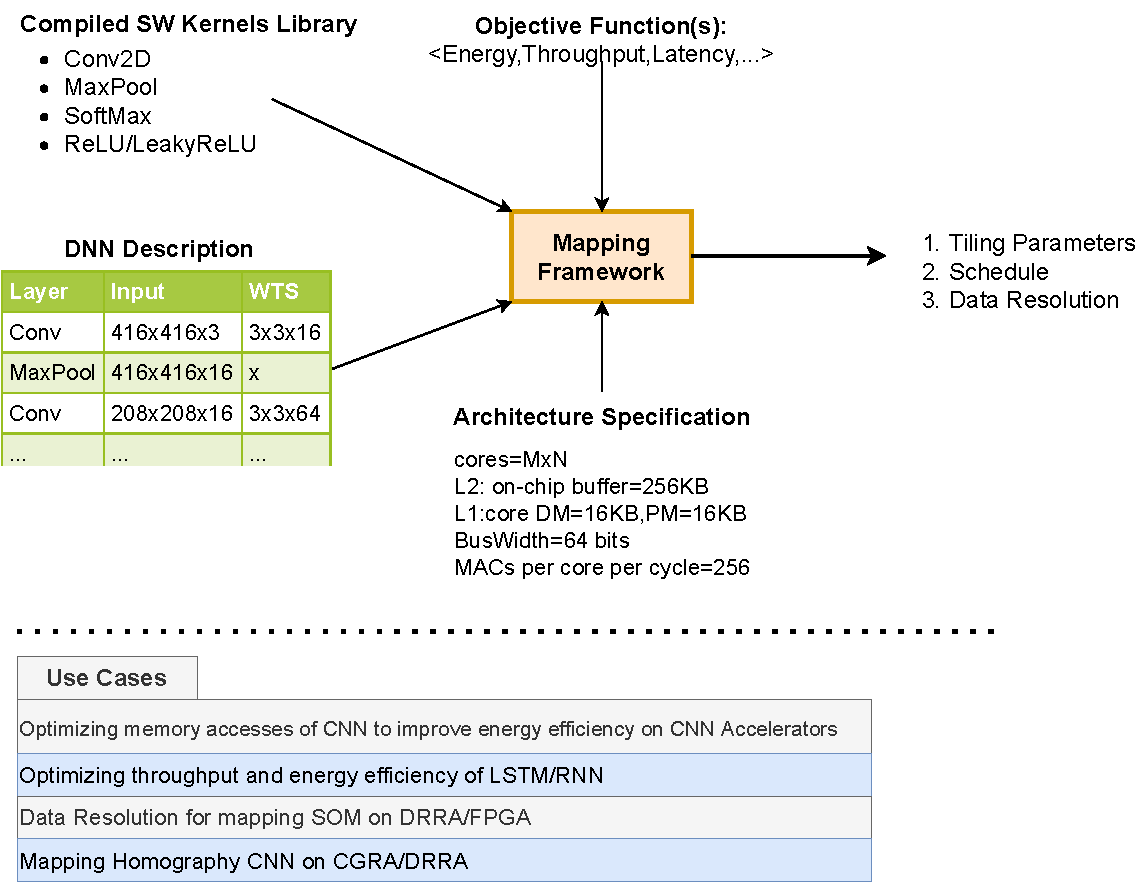
\includegraphics[width=0.7\linewidth]{./images/blockDiagram}
	\caption{Mapping DNN on coarse grain parallel architectures}
	\label{fig:introduction}
\end{figure}

\begin{enumerate}
	\item We propose a model that precisely estimates the off-chip memory accesses and the energy consumption of the DNN's layers, while taking into account the accelerator's architectural parameters.
	\item We propose an approach that determines the optimal partitoning of the DNN layers for reducing the off-chip memory accesses and energy consumptions. We analytically express the off-chip memory accesses of DNNs  using the layer shapes and tiling parameters and express it as a constraint optimization problem.
	\item We propose a novel data reuse approach to improve the performance and energy efficiency of recurrent neural networks (RNN). The proposed approach partitions the data and schedules the operations in a way that reduces the off-chip memory accesses of large matrices by half.
	\item We explore the limits of a neural network, self-organizing map (SOM), using different bit resolutions and the effect that it has on the accuracy, as well as the benefits that this low resolution can provide for a hardware architecture. 
%	\item We explore the design space of a self-organizing map (SOM) used for rapid and accurate identification of bacterial genomes. This is an important health care problem. 
	\item We do an in depth analysis of the reduction in resolution vs. loss in accuracy as the basis for designing a battery operated system where the area, power and performance are of critical importance.
\end{enumerate}

\section{Related Work}
We compare our approaches and show that our work significantly improves the performance and energy efficiency of DNN accelerators compared to the state of the art. To address the computational and energy efficiency of DNNs, several ASIC~\cite{conti2018chipmunk,wang2017accelerating,azari2020elsa} and FPGA based accelerators~\cite{chang2015recurrent,ferreira2016fpga,lee2016fpga,guan2017fpga,han2017ese} are proposed. The energy efficiency of DNN accelerators is critical for their widespread usage, and off-chip memory access is the key to improving energy consumption. Most of these works focused on improving energy efficiency by reducing off-chip memory accesses. Figure~\ref{fig:dataEnergyRelatedWork} shows broad categories of state of the art approaches that aim to improve energy efficiency of DNN accelerators by reducing the off-chip memory accesses.
\begin{figure}[!htb]
	\centering
	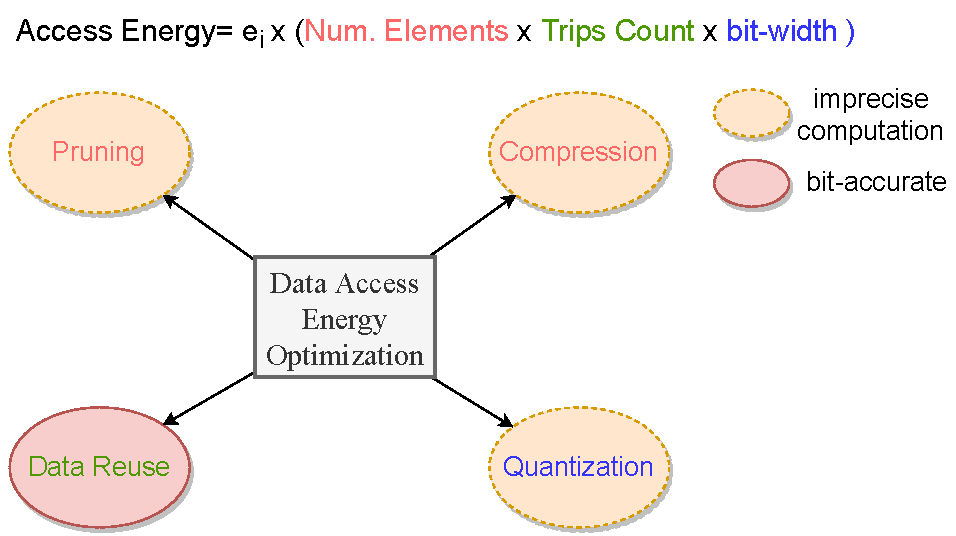
\includegraphics[width=0.4\textwidth]{./images/dataEnergyOptRelatedWork}
	\caption{Energy efficiency optimization approaches}
	\label{fig:dataEnergyRelatedWork}
\end{figure}

Some approaches~\cite{lee2016fpga, rybalkin2018finn, ferreira2016fpga} used on-chip memory to store all the weights. Sizes of weights in recent multi-layer LSTM models can be several MB's, and using large on-chip memory is expensive. These approaches are not scalable and effective only for small LSTM models. The proposed approach is independent of model size and effective for large LSTM models.

Several approaches used the fact that neural networks are error-tolerant and have lots of redundancy. They used the quantization and pruning techniques to compress the models' size. Approaches~\cite{ferreira2016fpga,wang2018c} used 18-bit, Chang et al.~\cite{chang2015recurrent} used 16-bit, Han et al.~\cite{han2017ese} used 12-bits precision for storing the inputs and weights, Lee et al.~\cite{lee2016fpga} used 8-bit inputs and 6-bits for weights to reduce the model size. The proposed approach is orthogonal to the quantization techniques and can be integrated with different quantization techniques to reduce the memory accesses further. 

Han et al.~\cite{han2017ese} used pruning to compress the model. However, pruning results in irregular network structure, and the sparse matrix require additional computational and storage resources and causes unbalanced load distribution. To overcome this Wang et al.~\cite{wang2018c} used block-circulant matrices representations to compress the LSTM/RNN model and to eliminate irregularities resulted from compression. Some approaches (\cite{park2019balancing,han2017ese,park2018maximizing}) used load balance aware pruning techniques to overcome the unbalanced load distribution problem. Quantization and pruning approaches impacts the accuracy of the networks and may not be suitable where accuracy is at priority. 

The other line of works reduced the memory accesses without compromising the accuracy of the network by applying the data-reuse techniques. Que et al.~\cite{que2019efficient} proposed a blocking-batching scheme to reuse the LSTM weights fetched from external memory. Park et al.(~\cite{park2020time}) proposed a time step interleaved weight reuse scheme (TSI-WR). 

\section{Off-Chip Memory Access Optimizations for CNN}
\subsection{Introduction}
CNNs perform compute and memory intensive operations.  To speed up the performance, CNN accelerators have large number of processing units (PE). 
CNNs have large amount of parallelism. However, limited on-chip memory, leads to repeated accesses from the off-chip memory and results in large volume of off-chip memory accesses. This lowers the resource utilization due to limited memory bandwidth and degrades energy efficiency significantly. 
\begin{figure}[!htb]
	\centering
	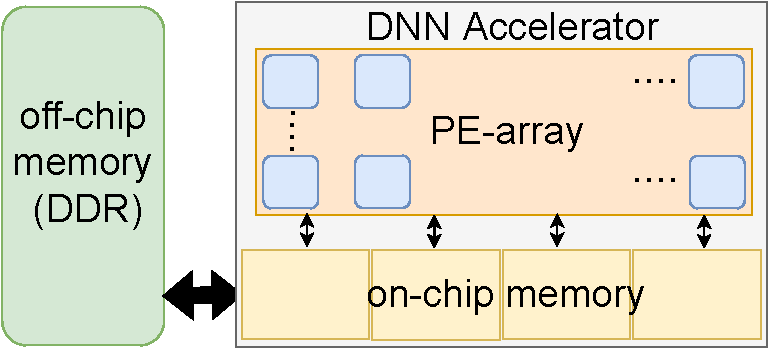
\includegraphics[width=0.4\textwidth]{DNNAccelerator}
	\caption{Typical DNN accelerator architecture}
	\label{fig:dnnAccelerator}
\end{figure}
To fit the layer data into on-chip memory, CNN accelerators apply loop tiling to partition the layer data into small tiles. Loop tiling is a compiler  technique~\cite{aho2006compilers} that partitions the loop iteration space and large arrays into smaller tiles to increase the data locality and ensures that data fits into smaller memories. The tile dimensions significantly impacts the off-chip memory accesses~\cite{zhang2015optimizing, Li2018SmartShuttleOO}. 
Determining optimal tile dimensions requires analyzing off-chip memory accesses for different tile dimensions. Memory accesses also depend on the architectural parameters of the accelerator like bus width and data alignment. We have proposed an approach that considers architectural parameters to compute the off-chip memory accesses accurately and determines the optimal tile dimensions and data reuse scheme for CNN layers.
\subsection{Related Work}
To meet the computation and energy demands of CNNs, researchers have proposed efficient accelerators~\cite{gokhale2014240,8742284,alwani2016fused, Chen2016EyerissAS}. Zhang et al.~\cite{zhang2015optimizing} and Li et al.~\cite{Li2018SmartShuttleOO} used loop tiling to optimize the off-chip memory accesses. They expressed the off-chip memory access as a function of tile dimensions and layer shape. Zhang et al.~\cite{zhang2015optimizing} determined optimal tile dimensions by enumerating all the legal tile dimensions. To reduce the hardware design complexity, they determined a global optimal tile dimension and used a common data reuse scheme for all the layers. Li et al.~\cite{Li2018SmartShuttleOO} proposed a layer-wise adaptive data partitioning and scheduling scheme. However, previous approaches ignored the architectural parameters and address alignment, and assumed all tiles of the same dimensions have the same off-chip memory accesses. With these assumptions, the tile dimensions determined by previous apporaches lead to a suboptimal solution.

\subsection{Bus Width Aware Off-chip Memory Access Estimation}\label{sec:OffChipAccessModel}
The CNN accelerators use a wide data bus to access off-chip memory to meet the high memory bandwidth requirement~\cite{Chen2016EyerissAS,chen2014diannao}. If the number of bytes accessed from an off-chip memory address is not a multiple of bus width or the address is not aligned to the word boundary, it results in unused bytes lanes of the data bus. Figure~\ref{fig:AXI_AccesseOn64BitDataBus} illustrates memory accesses on a 64-bit data bus.  Fig.~\ref{fig:AXI_AccesseOn64BitDataBus}a shows a read transaction of 8 bytes from an aligned address and uses the full bus width. However, if only 5 bytes are read from an aligned address, as shown in \figurename~\ref{fig:AXI_AccesseOn64BitDataBus}b, 8 bytes are still accessed. If 5 bytes are read from an unaligned address, it results in 16 bytes of data access, as shown in Fig.~\ref{fig:AXI_AccesseOn64BitDataBus}d. The unused byte lanes do not carry any useful data, but they contribute to overall energy consumption. The length of the data read should be chosen such that bus utilization is high, and off-chip memory accesses and energy consumption are minimized.
\begin{figure}[!htb]
	\centering
	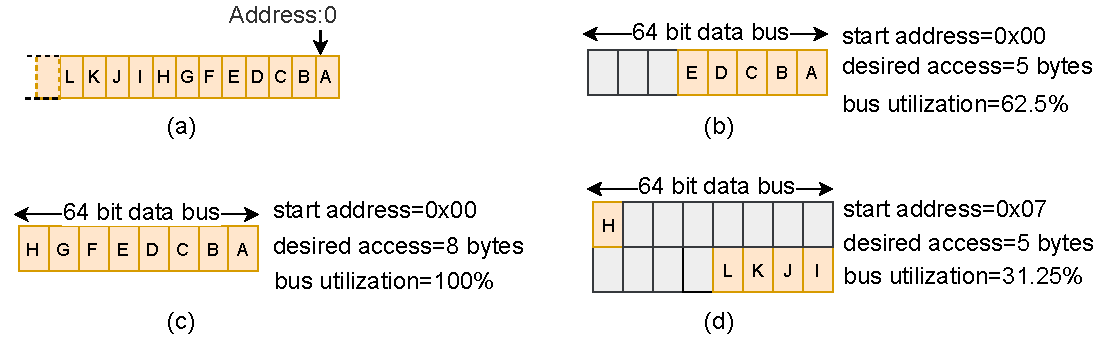
\includegraphics[width=0.7\textwidth]{./images/BurstTranscationOnAXI}
	\caption{Off-chip memory accesses on 64-bit wide data bus}
	\label{fig:AXI_AccesseOn64BitDataBus}
\end{figure}
To estimate the performance and energy efficiency, we have developed an offline model that estimates the off-chip memory accesses while taking into account the data alignment and memory bus width.

\subsection{Optimal data partitioning for CNNs}
Fig.~\ref{fig:partitioningDataUsingTiling} shows a CL data stored in off-chip memory and its tiles in the accelerator's on-chip buffer.
\begin{figure}[!htb]
	\centering
	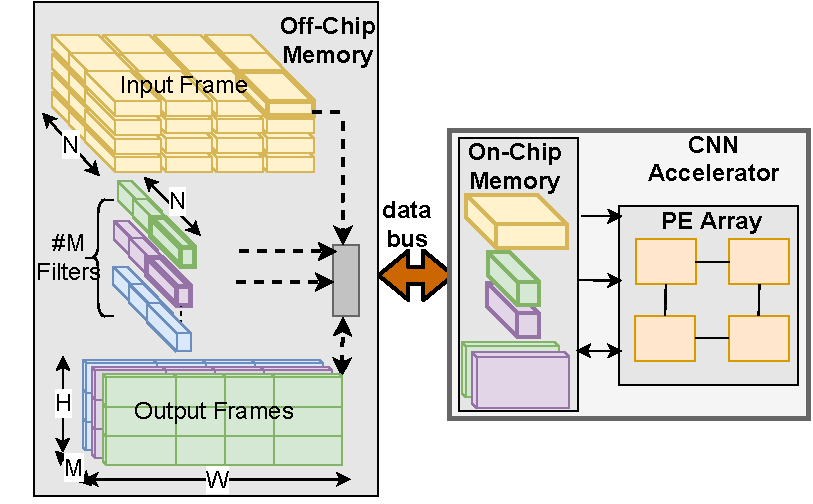
\includegraphics[width=0.5\textwidth]{images/AboutTheCNNTiles.pdf}
	\caption{CNN layer tiles in off-chip and on-chip memory}
	\label{fig:partitioningDataUsingTiling}
	\vspace{-1.0em}
\end{figure}
The off-chip memory access of 3D data can be computed as following
\begin{align}\label{eq:BasicOffChip3DDataAccess}
	\numBytesOffChip_{3D}{=}r{\times} \sum_{t=1}^{N_{tiles}}{\numBytesOffChip_{t}}
\end{align}
where $N_{tiles}$ is the number of tiles. $r$ and $\numBytesOffChip_{t}$ are the trips count and the number of bytes accessed from off-chip memory of the $t^{th}$ tile, respectively.  The trips count $r$ depends on the data reuse scheme, and $\numBytesOffChip_{t}$  is computed using the model described in section~\ref{sec:OffChipAccessModel}

Tiles of \textit{ifm, ofm} and \textit{wts} reside in on-chip memory.If the on-chip memory buffer size is $\BuffSize$, and $V_{ifm}, V_{ofm}, \text{and }V_{wts}$ are the size of \textit{ifm, ofm}, and \textit{wts} tiles, respectively, then constraints on tile dimensions are
\begin{align}\label{eq:onChipConstraint}
		(V_{ifm}{+}V_{wts}{+}V_{ofm})\cdot{DW}\leq \BuffSize 
\end{align}
Determining the tile dimensions which minimize the off-chip memory accesses, is a constraint optimization problem. The  number of bytes accessed from off-chip memory and the constraints \eqref{eq:onChipConstraint} are non-linear functions of tile dimensions and solving it is non-trivial.

We propose an approach to determine the optimal tile dimensions by computing the number of bytes accessed from off-chip memory ($\numBytesOffChip$) at all the feasible points using section~\ref{sec:OffChipAccessModel}. Our approach determines the optimal tile dimensions for each layer for different data reuse schemes and it can be configured for different on-chip memory sizes, bus widths, and data bit width. 
\subsection{Results}
We experimented with three popular CNN networks, AlexNet~\cite{krizhevsky2012imagenet}, VGG16~\cite{simonyan2014very}, and ResNet~\cite{he2016deep} having 8, 16, and 50 layers, respectively, with varying layer shapes and using filters of dimensions $1{\times}1$, $3{\times}3$, $5{\times}5$, $7{\times}7$, and $11{\times}11$. To compare the results with other approaches, we have used the on-chip buffer size of 108 KB, batch size of 3 for VGG16, and 4 for ResNet and AlexNet. Figure~\ref{fig:EffectOnLatency} shows the comparison of the proposed approach with SmartShuttle (SS)~\cite{Li2018SmartShuttleOO} for VGG16. The SS approach determines the tile dimensions and data reuse scheme adaptively for each layer to minimize the data size (volume) accessed from off-chip memory. 
\begin{figure}[!htb]
	\centering
	\subfloat[VGG16: Energy and latency efficiency]
	{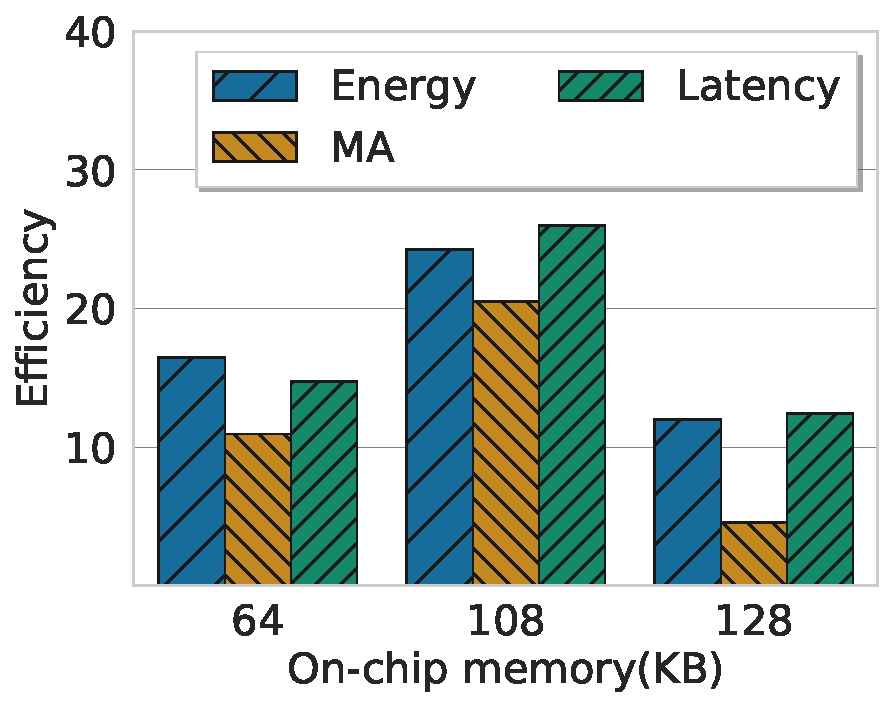
\includegraphics[width=0.3\textwidth]{energy_VGG16_DW8_BW64.pdf}
		\label{fig:VGG16EnergyEfficiency}}
	\hfil
	\subfloat[$\numBytesOffChip_{VGG16}$: Varying on-chip buffer sizes]
	{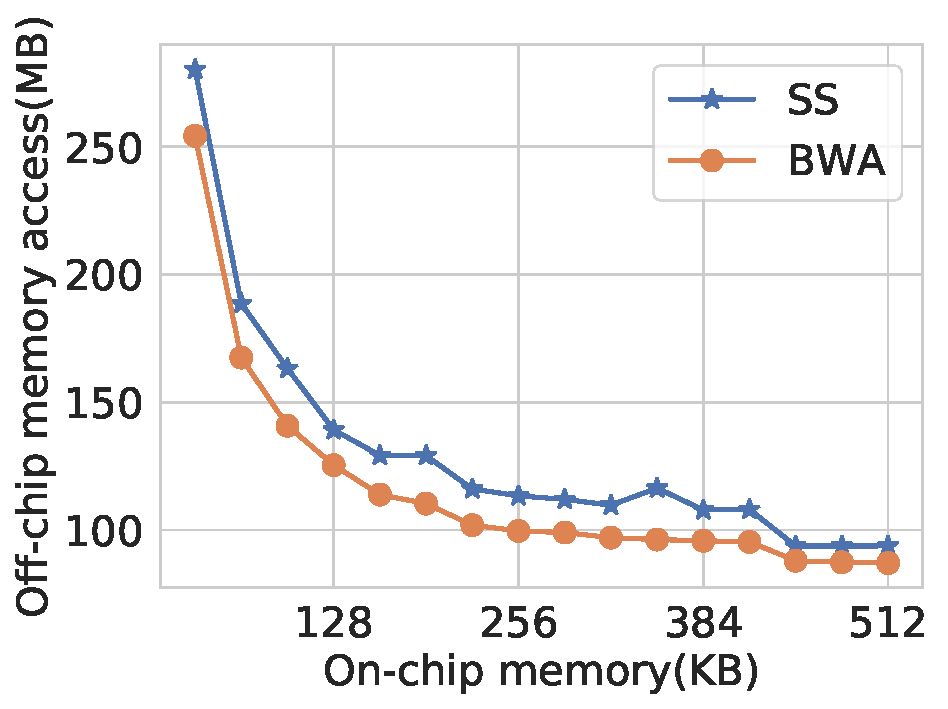
\includegraphics[width=0.3\textwidth]{VGG16_mem0_batch3_bw8_dW8_AD0.pdf}
		\label{fig:VGG16OnChipMemoryEffect}}
	\hfil
	\subfloat[VGG16: Fully connected layers]
	{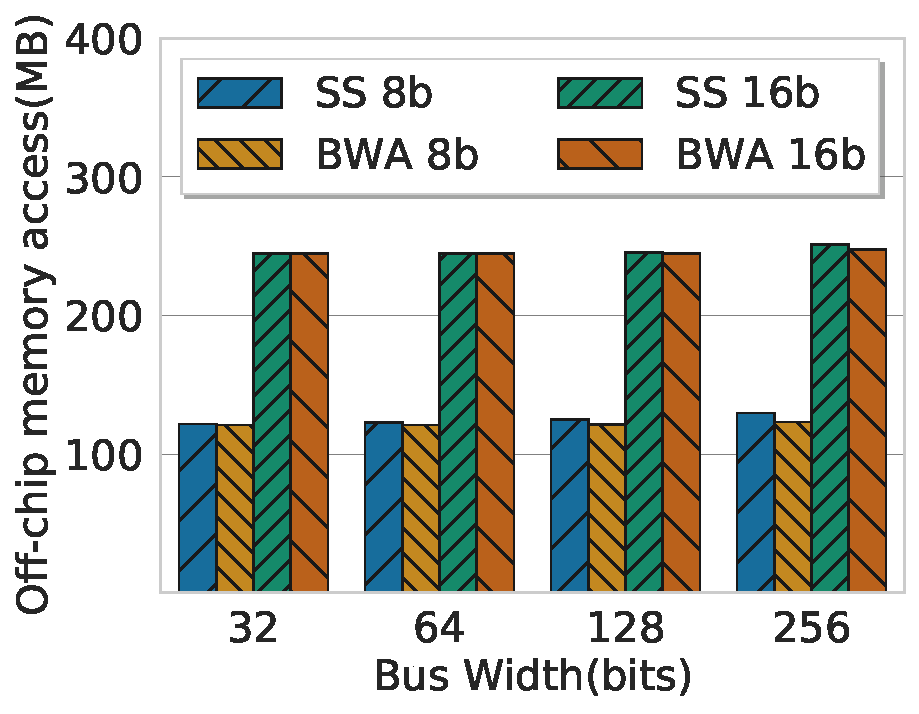
\includegraphics[width=0.3\textwidth]{VGG16_mem108_batch3_bw0_dW0_AD0_FC.pdf}
		\label{fig:VGG16FCLayer}}
	\hfil
	\caption{Latency and off-chip memory access. BWA: Bus Width Aware, SS:SmartShuttle}
	\label{fig:EffectOnLatency}
	\vspace{-1.0em}
\end{figure}
\subsubsection{Latency And Energy Analysis}
\figurename{~\ref{fig:VGG16EnergyEfficiency}} show the energy, off-chip memory accesses, and latency efficiency achieved using the BWA compared to the SS approach for VGG16 for 8 bits data width and 64 bits bus width. Using our FPGA implementation, we measured the memory access latencies and execution time for CLs to estimate the energy efficiency of the BWA approach compared to the SS approach. We observed that the changes in energy and latency are proportional to the changes in memory access. This observation confirms that off-chip memory access dominates the energy consumption of the CNN accelerators.
\subsubsection{On-chip Memory Size}
The size of the on-chip memory constrains the tile dimensions. Larger on-chip memory can accommodate bigger tiles which reduces the trips and number of off-chip memory access transactions. \figurename{~\ref{fig:VGG16OnChipMemoryEffect}} shows off-chip memory access for VGG16. Off-chip memory access reduces with increasing on-chip memory size for both approaches. However, the BWA approach performs better than SS for all the on-chip memory sizes.
\subsubsection{Impact of Bus Width on $\numBytesOffChip$ of FCLs}
In FCLs, the height and width of tiles and data are the same. Tiles in FCL can be accessed from off-chip memory using a single transaction which results in fewer transactions in FCLs compared to CLs. Whereas in CLs, multiple transactions are required to access different rows of the tiles. Thus the impact of bus width is less on $\numBytesOffChip$ of FCLs as compared to CLs. \figurename~\ref{fig:VGG16FCLayer} shows the off-chip memory accesses of FCLs of VGG16 for 8 bits data width. BWA reduces $\numBytesOffChip_{VGG16}^{FC}$ by 1\%, 2\%, 3\%, and 4\% on 32, 64, 128, and 256 bits wide buses, respectively. 
\section{Data reuse approach for RNNs}
\subsection{Introduction}
Many applications involve sequential data processing and time-series predictions, e.g., natural language processing, speech recognition, video activity recognition, sentiment classification. Processing sequential data requires remembering the contextual information from previous data. Recurrent neural networks (RNNs) are deep learning algorithms specialized in handling such problems by maintaining an internal state based on previously seen data. LSTMs \cite{hochreiter1997long} are variants of RNNs designed to handle long-range dependencies by storing useful information about previous inputs for a long duration. 

%Customized accelerators are proposed to speed up the computations of LSTM. These accelerators have limited on-chip memory, specifically the accelerators targeted for embedded devices. 
LSTM computations involve multiple matrix-vector multiplications, and these matrix-vector multiplications are performed several times. The size of these matrices can be significant in several MB's and often exceed the size of the accelerator's on-chip memory. These matrices are partitioned into blocks and accessed from off-chip memory repeatedly by the accelerator, which results in a large volume of off-chip memory accesses and energy consumption. The high energy consumption limits the usage of these accelerators on embedded devices.

Typically the computations of LSTM cell is described by the following equations
\begin{align}\label{eq:lstmEqs}
	\begin{split}
		&i{=}{\sigma}(W^i{\cdot}x_t{+}R^i{\cdot}h_{t-1}{+}b^i)\\
		&f{=}{\sigma}(W^f{\cdot}x_t{+}R^f{\cdot}h_{t-1}{+}b^f)\\
		&g{=}{\tanh}(W^g{\cdot}x_t{+}R^g{\cdot}h_{t-1}{+}b^g)\\
		&o{=}{\sigma}(W^o{\cdot}x_t{+}R^o{\cdot}h_{t-1}{+}b^o)\\
		&c_{t}{=}f{\odot}c_{t-1}{+}i{\odot}g\\
		&h_{t}{=}o{\odot}{\tanh}(c_t)
	\end{split}	
\end{align}
where $x_t$ is the input, $h_t$ is the hidden state, and $c_t$ is the cell state at time $t$. $i,f,g,o$ are the computed gate values. $\odot$ denotes the element-wise multiplications. $W^j$ and $R^j$ are the input and hidden state weight matrices, and $b^j$ is the bias vector, learned during the training process, where $j\in\{i,f,g,o\}$. The dimension of $h_t$ is referred to as the number of hidden states of the LSTM ($N$). 
At every time step, $x_t$ is taken as input, and cell state ($c_t$) and hidden state ($h_t$) are computed using~\eqref{eq:lstmEqs}. The dependency of $h_t$ on $h_{t-1}$ and $c_{t-1}$ prevents the parallel processing of multiple time steps and limits the data reuse. 

Figure{~\ref{fig:introToApproach}} shows the LSTM cell computations for two consecutive time steps using  conventional and the proposed approach. To compute the hidden state vector $h_t$, conventional approaches accesses $R$ matrix at each time step $t$, as shown in Fig.{~\ref{fig:introA}}. Accessing the weights at each time step results in large volume of off-chip memory accesses. 
\begin{figure}[!htb]
	\centering
	\subfloat[Conventional approaches: $R$ matrix is accessed at each time step.]
	{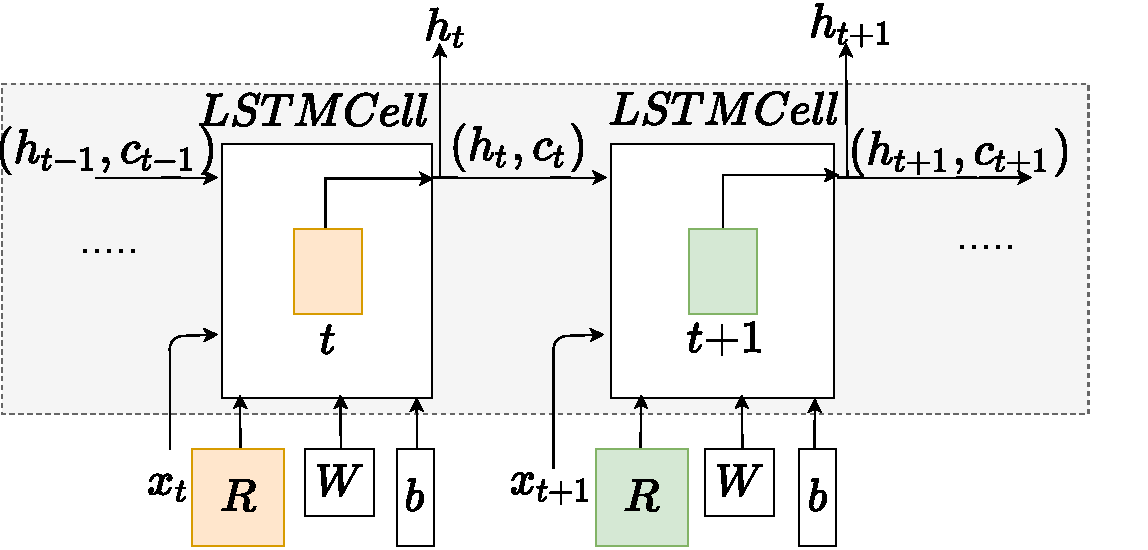
\includegraphics[width=0.4\textwidth]{introA.pdf}
		\label{fig:introA}}
	\hfil
	\subfloat[Proposed approach: $R$ matrix accesses are reduced by half. ]
	{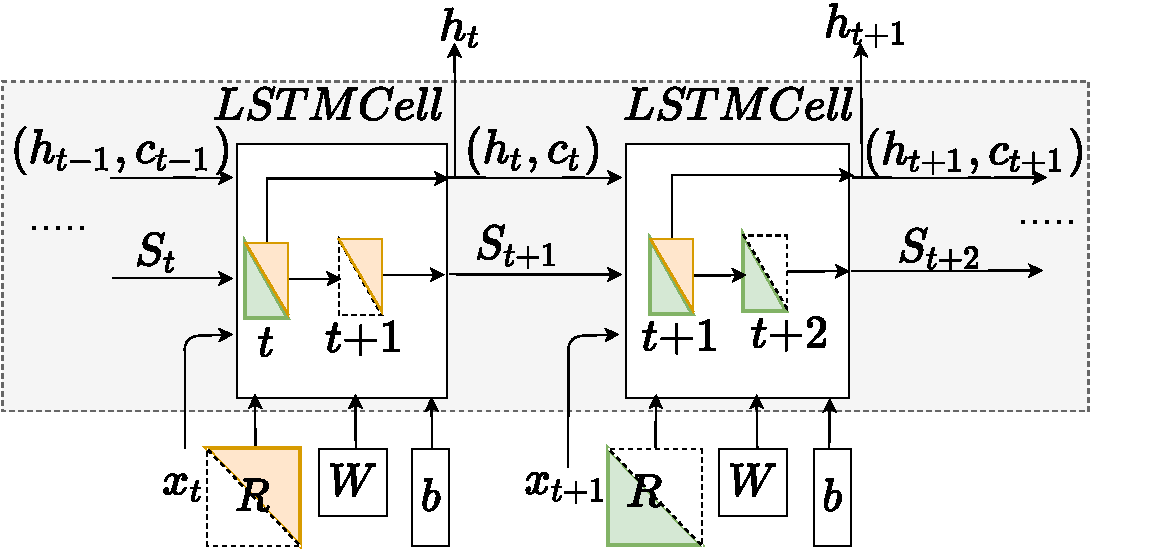
\includegraphics[width=.4\textwidth]{introB.pdf}
		\label{fig:introB}}
	\hfil	
	\caption{LSTM cell computations for consecutive time-steps showing the weight accesses.}
	\label{fig:introToApproach}
	\vspace{-1.0em}	
\end{figure}
\subsection{Previous Work}
Que et al.~\cite{que2019efficient} proposed a blocking-batching scheme to reuse the LSTM weights fetched from external memory. Their approach reuses the weights of $W$ matrix on a group of input vectors, by processing those input vectors as a batch. The input vectors in the same batch share the same weight matrices ($W$). However, it is difficult to collect required number of input vectors. As the LSTM cell states computations depend on cell states of the previous time-step, benefit of their batching schemes is limited to $W$ matrix. Reusing weights of $R$ across different time-steps has not been successful because of the state dependency.

Park et al.(~\cite{park2020time}) proposed a time step interleaved weight reuse scheme (TSI-WR) which reuses the weights of $R$ matrix between two adjacent time steps by performing computations in a time-interleaved manner. Their approach logically partitions the $R$ matrix into blocks. A block is accessed from off-chip memory to compute the two consecutive hidden state vectors partially. However, their approach do not fully exploit the data reuse, and several weights are accessed repeatedly from the off-chip memory. In addition, the data reuse in TSI-WR approach depends on the on-chip storage size which limits the benefits of their approach.
\subsection{Proposed data reuse approach}
We proposes an approach that reduces off-chip memory accesses by splitting the computation in two. At each time step, while the computations of a hidden state vector of one time step $h_t$ completes, partial computation of next time step ($S_{t+1}$) is also performed by reusing the weights.
Our approach schedules the computations in a way that reuses all the weights of $R$ between two adjacent time steps. The data reuse in our approach is independent of on-chip buffer sizes which makes it suitable for accelerators with very small on-chip memory.

The proposed data reuse approach splits and combines the LSTM cell computations in a way that reduces the off-chip memory accesses of hidden state matrices by 50\%. The computation of the $h_t$ can be expressed as shown below
\begin{align}\label{eq:h_{t}}
	h_{t}[k] &= F( S_{t}[k]+q_{t}[k])
\end{align}
where $F$ is a non-linear function. $q_{t}$ is computed as $W{\cdot}x_t{+}b$ and its computations are independent of previous step cell states. $S_{t}[k]$ is the sum of $N$ product terms as shown below,
\begin{align}
	S_{t}[k] = \sum_{n=0}^{N-1}R[k][n]\cdot h_{t-1}[n]
\end{align}
$S_{t}[k]$ can be computed as a sum of the following two partial sums $S_{t}^{L}[k]$ and $S_{t}^{U}[k]$
\begin{align}      
	S_{t}^{L}[k] &= \sum_{n=0}^{k}R[k][n]\cdot h_{t-1}[n] \label{eq:S_L_{t}}\\
	S_{t}^{U}[k] &= \sum_{n=k+1}^{N-1}R[k][n]\cdot h_{t-1}[n] \label{eq:S_U_{t}}
\end{align}
Equation~\eqref{eq:S_L_{t}} uses the lower-diagonal and diagonal elements of $R$ ($R^L$), and~\eqref{eq:S_U_{t}} uses the upper diagonal elements of $R$ ($R^U$). 
\begin{figure}[!htb]
	\centerline{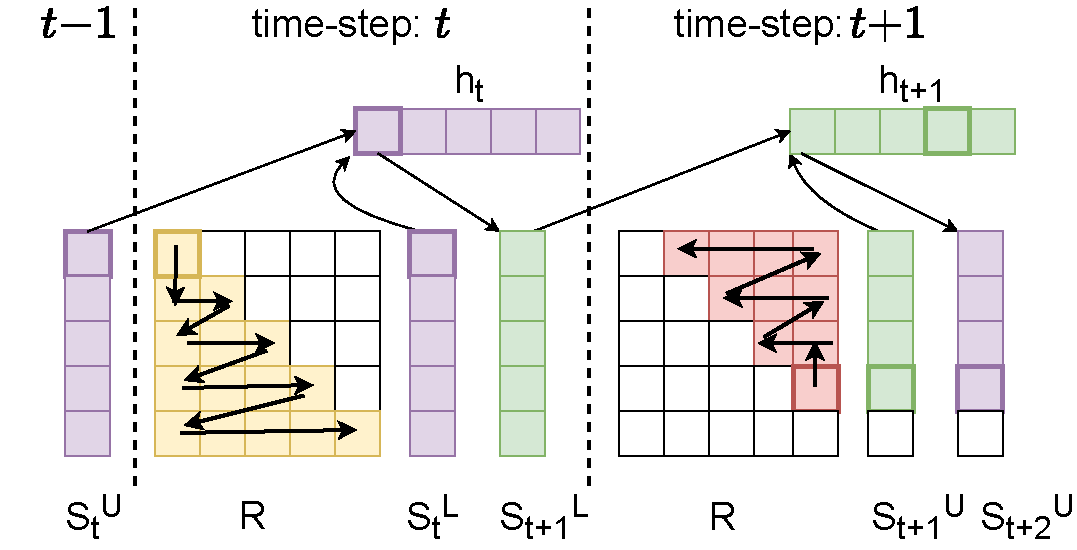
\includegraphics[width=0.5\textwidth]{TwoTimeSteps.pdf}}
	\caption{Splitting the hidden state vector computations into partial sums}
	\label{fig:TwoTimeStepsComputation}
	\vspace{-1.0em}	
\end{figure}
As shown in \figurename{~\ref{fig:TwoTimeStepsComputation}}, $R^L$ and $R^U$ are accessed in consecutive time steps and reused in the partial sum computations of two steps. At time step $t$, $S_t^U$ and $h_{t-1}$ are the inputs from the previous time step, and $R^L$ is reused to compute the partial sums $S_{t}^{L}$ and $S_{t+1}^L$. Input $S_{t}^{U}$ is added to $S_{t}^{L}$ to compute $h_{t}$, and $S_{t+1}^L$ is passed to $(t{+}1)^{th}$ step computations.
In the same way, at time step $t{+}1$, $R^U$ is reused to compute $S_{t+1}^{U}$ and $S_{t+2}^{U}$. Elements of $R^L$ are accessed from top to bottom, left to right, while elements of $R^U$ are accessed in the reverse order to satisfy the dependencies. As shown in~\figurename{~\ref{fig:TwoTimeStepsComputation}}, the proposed approach accesses the weight matrix $R$ once, to compute the output of two consecutive time steps $h_{t}$ and $h_{t+1}$. 
\subsection{Results}
We have compared our approach with conventional approaches and TSI-WR approach~\cite{park2020time}. Conventional approaches access the hidden state weight matrices $R$ at each step from the off-chip memory. We have used the same on-chip buffer size to store the weight matrices ($4{\times}B{^2}$) to perform a fair comparison. The proposed approach requires additional on-chip memory ($4N{+}4B$) to store the four partial sum and temporary vectors.
We have experimented with LSTM models used in speech recognition (for TIMIT~\cite{garofolo1993timit}) and character level Language Modelling (LM)~\cite{sundermeyer2015feedforward}.
\begin{figure}[!htb]
	\centering
	\subfloat[]
	{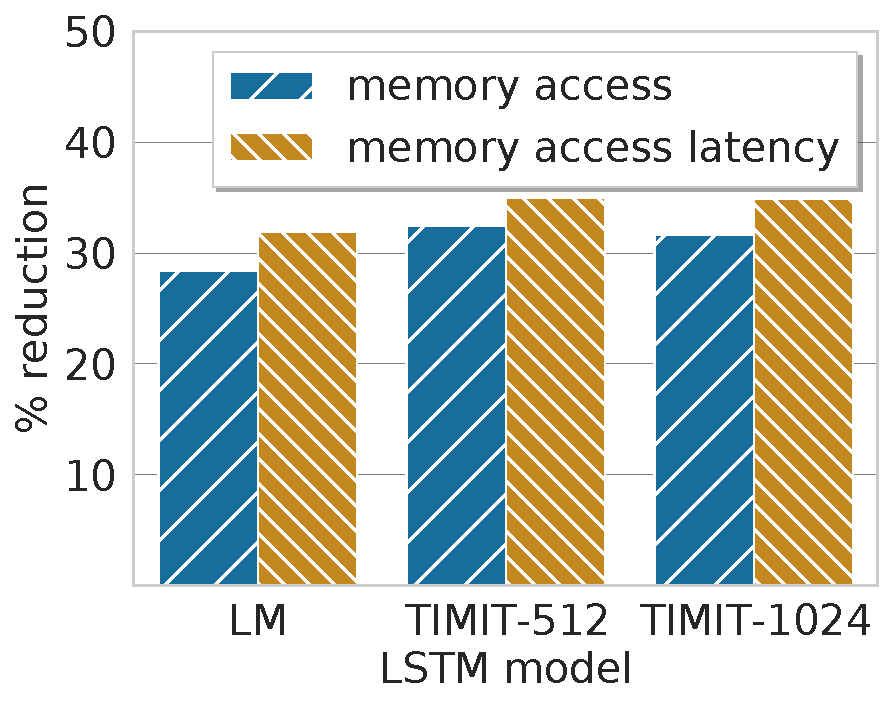
\includegraphics[width=0.3\textwidth]{memAccessForModels.pdf}
		\label{fig:memAccessForModels}}
	\hfil
	\subfloat[]
	{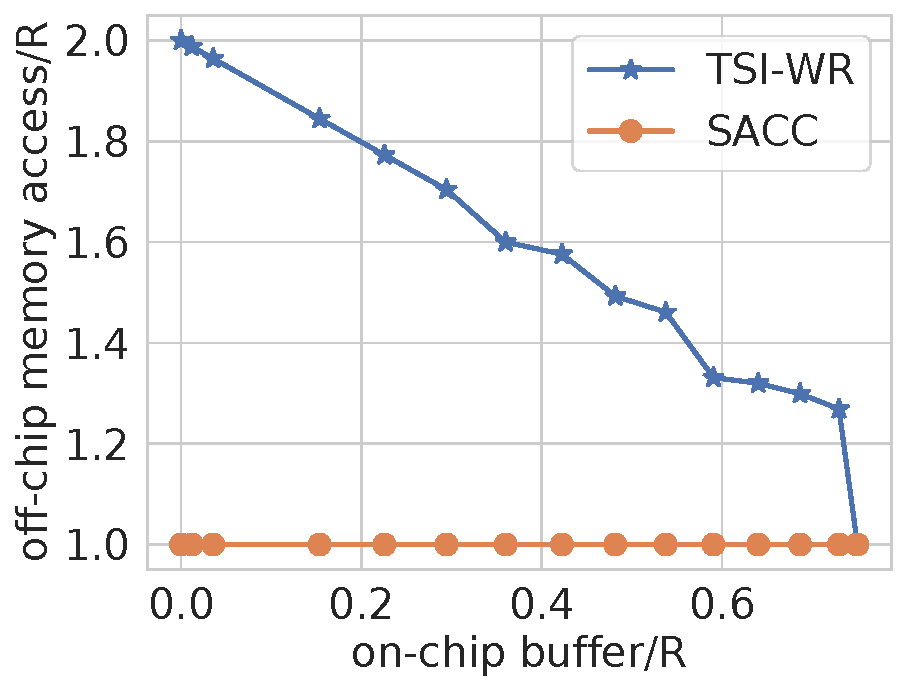
\includegraphics[width=0.3\textwidth]{tsiwrComparison.pdf}
	\label{fig:compareWithTSIWR}}
	\subfloat[]
	{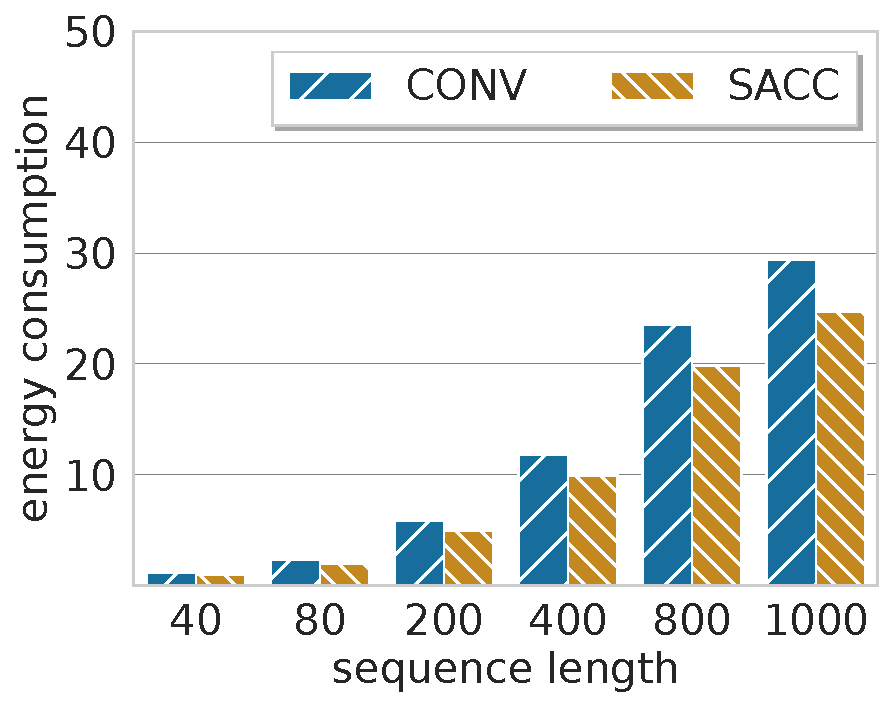
\includegraphics[width=0.3\textwidth]{energyTIMIT1024.pdf}
		\label{fig:energyEfficiencyForSeqLengths}}
	\caption{(a) off-chip memory access and latency (b) Off-chip memory access comparison between TSI-WR and SACC approach for two consecutive time steps. (c) normalized energy. CONV: conventional}	\label{fig:compareMemAccessAndRunTime}
	\vspace{-1.0em}	
\end{figure}
\subsubsection{Memory Accesses}
\figurename{~\ref{fig:memAccessForModels}} shows the proposed approach's reduction in off-chip memory accesses compared to conventional approaches. The proposed approach reduces the memory accesses of the $R$ matrices by half. Total memory accesses, including $R, W$, and $b$, for LM and TIMIT models reduce by 28\% and 32\%, and memory access latencies reduce by 29\% and 31\%, respectively.
The proposed approach reduces the run-time by 12.8\% and 16\% for LM and TIMIT models. 
\subsubsection{Comparison with TSI-WR}
\figurename{~\ref{fig:compareWithTSIWR}} compares the off-chip memory accesses of the SACC and the TSI-WR approaches using the simulation results. The performance of the TSI-WR approach depends on on-chip buffer sizes. TSI-WR reduces 50\% off-chip memory accesses when the on-chip buffer size is 70\% of the $R$ matrix. The proposed approach reduces R's memory access by 50\%, irrespective of the on-chip buffer size.
\subsubsection{Energy Efficiency}
We computed the energy consumption using the design power reported by the Vivado synthesis tool, execution time, and off-chip memory accesses. \figurename{~\ref{fig:energyEfficiencyForSeqLengths}} shows the normalized energy consumption of the conventional and the proposed approach for TIMIT-1024. Due to the reduction in the run-time and off-chip memory accesses, the SACC approach reduces the energy consumption on average by 13\% and 16\% for LM and TIMIT models.


\section{Optimizing SOMs using low bit-width}
\subsection{Introduction}
One of the popular low-power stategy is performing computations at reduced bit-widths. In some cases, this results in trading off accuracy for smaller power consumption. The benefits of doing this results in improved energy performance metrics in both the data path and in the memory path. This is because there is a reduction of the energy cost for data transfers, which usually dominates the total energy consumption for such systems. Machine learning tasks do have intrinsic error resilience and hence it is expected that bit-width reduction will work well. 

%In this work, we explore the impact of different bit resolutions on the accuracy, as well as the benefits that this low resolution can provide for a hardware architecture. We have done hardware implementation of SOM on FPGA, mapped on Xilinx Virtex7 485t chip, handcrafted for different bit width implementations to analyze the area vs energy trade off.

We explore the design space of a self-organizing map (SOM) used for rapid and accurate identification of bacterial genomes which is an important health care problem.  SOM has been implemented as an FPGA design and shown to have better computational efficiency compared to GPUs. To further lower the energy consumption, we exploit the robustness of SOM by successively lowering the resolution to gain further improvements in efficiency and lower the implementation cost without substantially sacrificing the accuracy. We do an in depth analysis of the reduction in resolution vs. loss in accuracy as the basis for designing a system with the lowest cost and acceptable accuracy. The objective of this method is to design a bacterial recognition system for battery operated clinical use where the area, power and performance are of critical importance. We demonstrate that with 39\% loss in accuracy in 12 bits and 1\% in 16 bit representation can yield significant savings in energy and area.

Prior work in \cite{Yang2018RiBoSOM} has introduced Self-organizing maps (SOM) for rapid genome identification. SOM uses a type of unsupervised learning called competitive ANN learning model. The model reduces the data dimensions and it clusters similar data together \cite{Kohonen2013}. A trained SOM network does not require to go through the whole DNA sequence to recognize the pathogen, but only requires a small part of its DNA. SOM can be highly parallelized and such parallel implementation have been proposed for synchoros VLSI design, custom FPGA and GPUs \cite{Yang2018RiBoSOM, Porrmann2006, McConnell2012}. Another important aspect of SOM and other ANN is their robustness. ANNs have been proven to work with low bit resolution without sacrificing much of their accuracy \cite{8056820}. In this work, we explore the limits of the SOM using different bit resolutions and the effect that it has on the accuracy of the SOM, as well as the benefits that this low resolution can provide for a hardware architecture. 

\subsection{Previous Work}
 An emerging design paradigm that is able to achieve better energy efficiency by trading off the quality (e.g., accuracy) and effort (e.g., energy) of computation is approximate computing ~\cite{Zhang2014}. Many modern applications, such as machine learning and signal processing, are able to produce results with acceptable quality despite most of the calculations being computed imprecisely~\cite{Ye2013}. The tolerance of imprecise computation in approximate computing  to acquire substantial performance gains and is the basis for a wide range of architectural innovations~\cite{Esmaeilzadeh2012}.


Earlier work in approximate computing was focused on the design of basic elements, such as approximate adders and logic~\cite{Gupta2012}.  Although, these techniques  adequately demonstrated the benefit of approximate computing,  the fixed functionality and low-level design limits further performance improvement. Additionally, many of these techniques use complementary metal-oxide-semiconductor (CMOS) technology. Innovations in   device technology  provide a great opportunity for radically different forms of architecture design~\cite{Venkataramani2012}.

One of the  popular low-power strategy implemented in custom designs consists in performing computations at reduced bit-widths. In some cases, this results in  trading off accuracy for smaller power consumption. The  benefits of doing this results in improved energy performance metrics in both the data path and in the memory path. This is because  there is a  reduction of the energy cost for data transfers, which usually dominates the total energy consumption for such systems. Machine learning tasks do have intrinsic error resilience  and hence it is expected that bit-width reduction will  work well Additionally, there is a body of literature that has demonstrated that high-precision computations are often unnecessary in presence of statistical algorithms~\cite{Moons2017,Zhang2015}. Znag et.al. report a less than 5\% of quality loss  obtained by simulation of the real hardware implemented in a 45nm CMOS technology. Gupta et. al. also present similar results where they train deep networks with 16 bits fixed-point number representations and stochastic rounding~\cite{Gupta2015}. Talathi et. al. show that  the best performance with reduced precision  can be  achieved with 8 bits weights and 16 bits activation, which, if reduced to 8 bits, results in  a 2\% drop in accuracy. Hashemi et. al. look at a broad range of numerical representations applied to ANNs in both inputs and network parameters and analyze the trade-off between accuracy and hardware implementation metrics and conclude that a wide range of approximation parameters are feasible with negligible degradation in performance~\cite{Hashemi2017}.

\subsection{Analyzing impact of low bit-width}
We have implemented SOM on FPGA, mapped on a Xilinx Virtex7 485t chip, of SOM for identification of bacterial genomes. A custom semi systolic array was hand crafted, for different bit width implementations, to analyze the area versus energy trade off.

Figure \ref{fig:algo} shows a high level schematic of the FPGA implementation of BioSOM and illustrates the key components in the design. The input is a $n$-bit vector. Each pair of bits in the input represents one of nucleotide A,C,G or T. Thus a 16-bit word contains 8 symbols.  The Neural Network weights are stored in BRAMs. Each neuron has 8 weights and each weight is stored as a fixed-point number. Bit width analysis is performed by varying the number of bits (8, 12, 16, 24 and 32) used to represent the weights.

\begin{figure}[!htb]
	\centering
	\subfloat[]
	{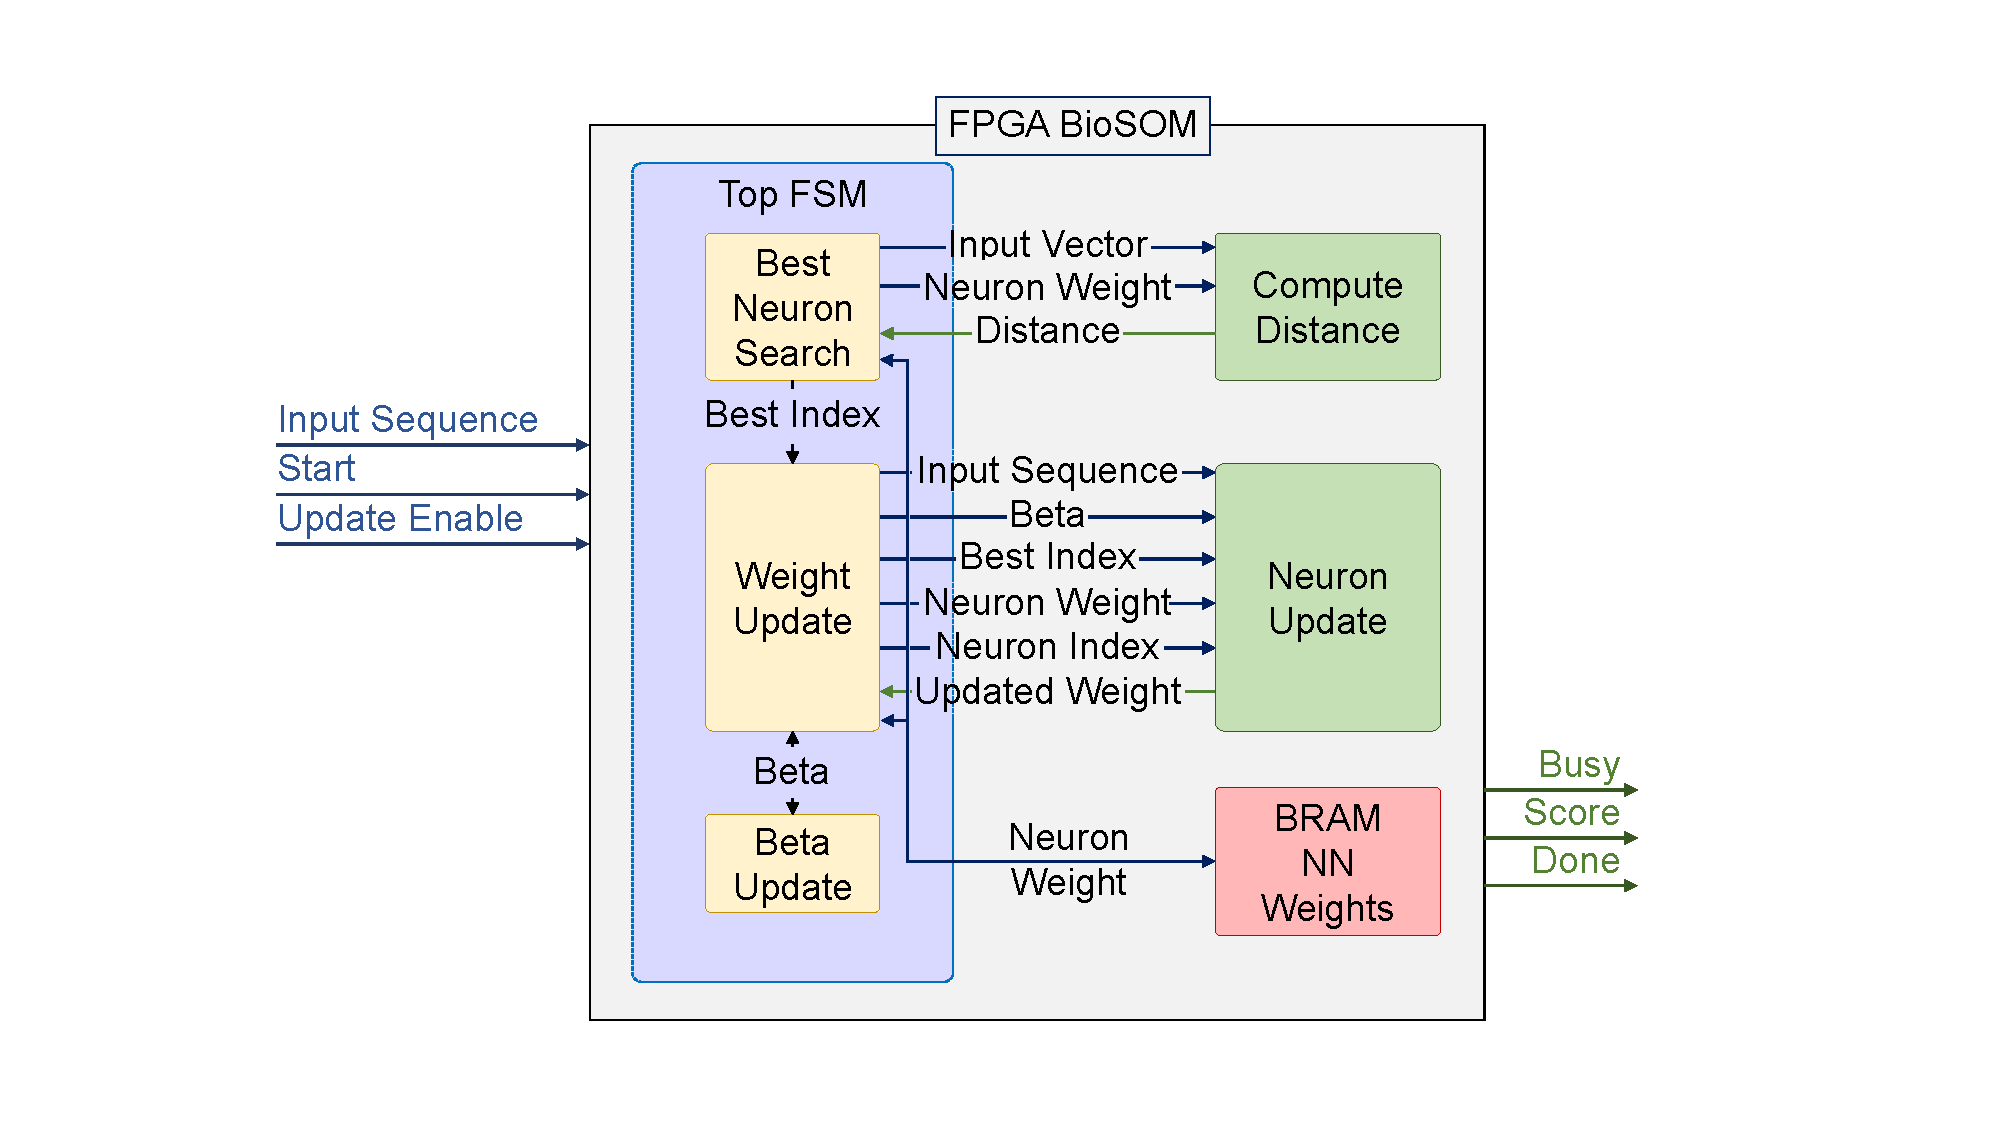
\includegraphics[width=0.48\textwidth]{./somResults/SOMDesignOne_v2}
		\label{fig:algo}}
	\hfil
	\subfloat[]
	{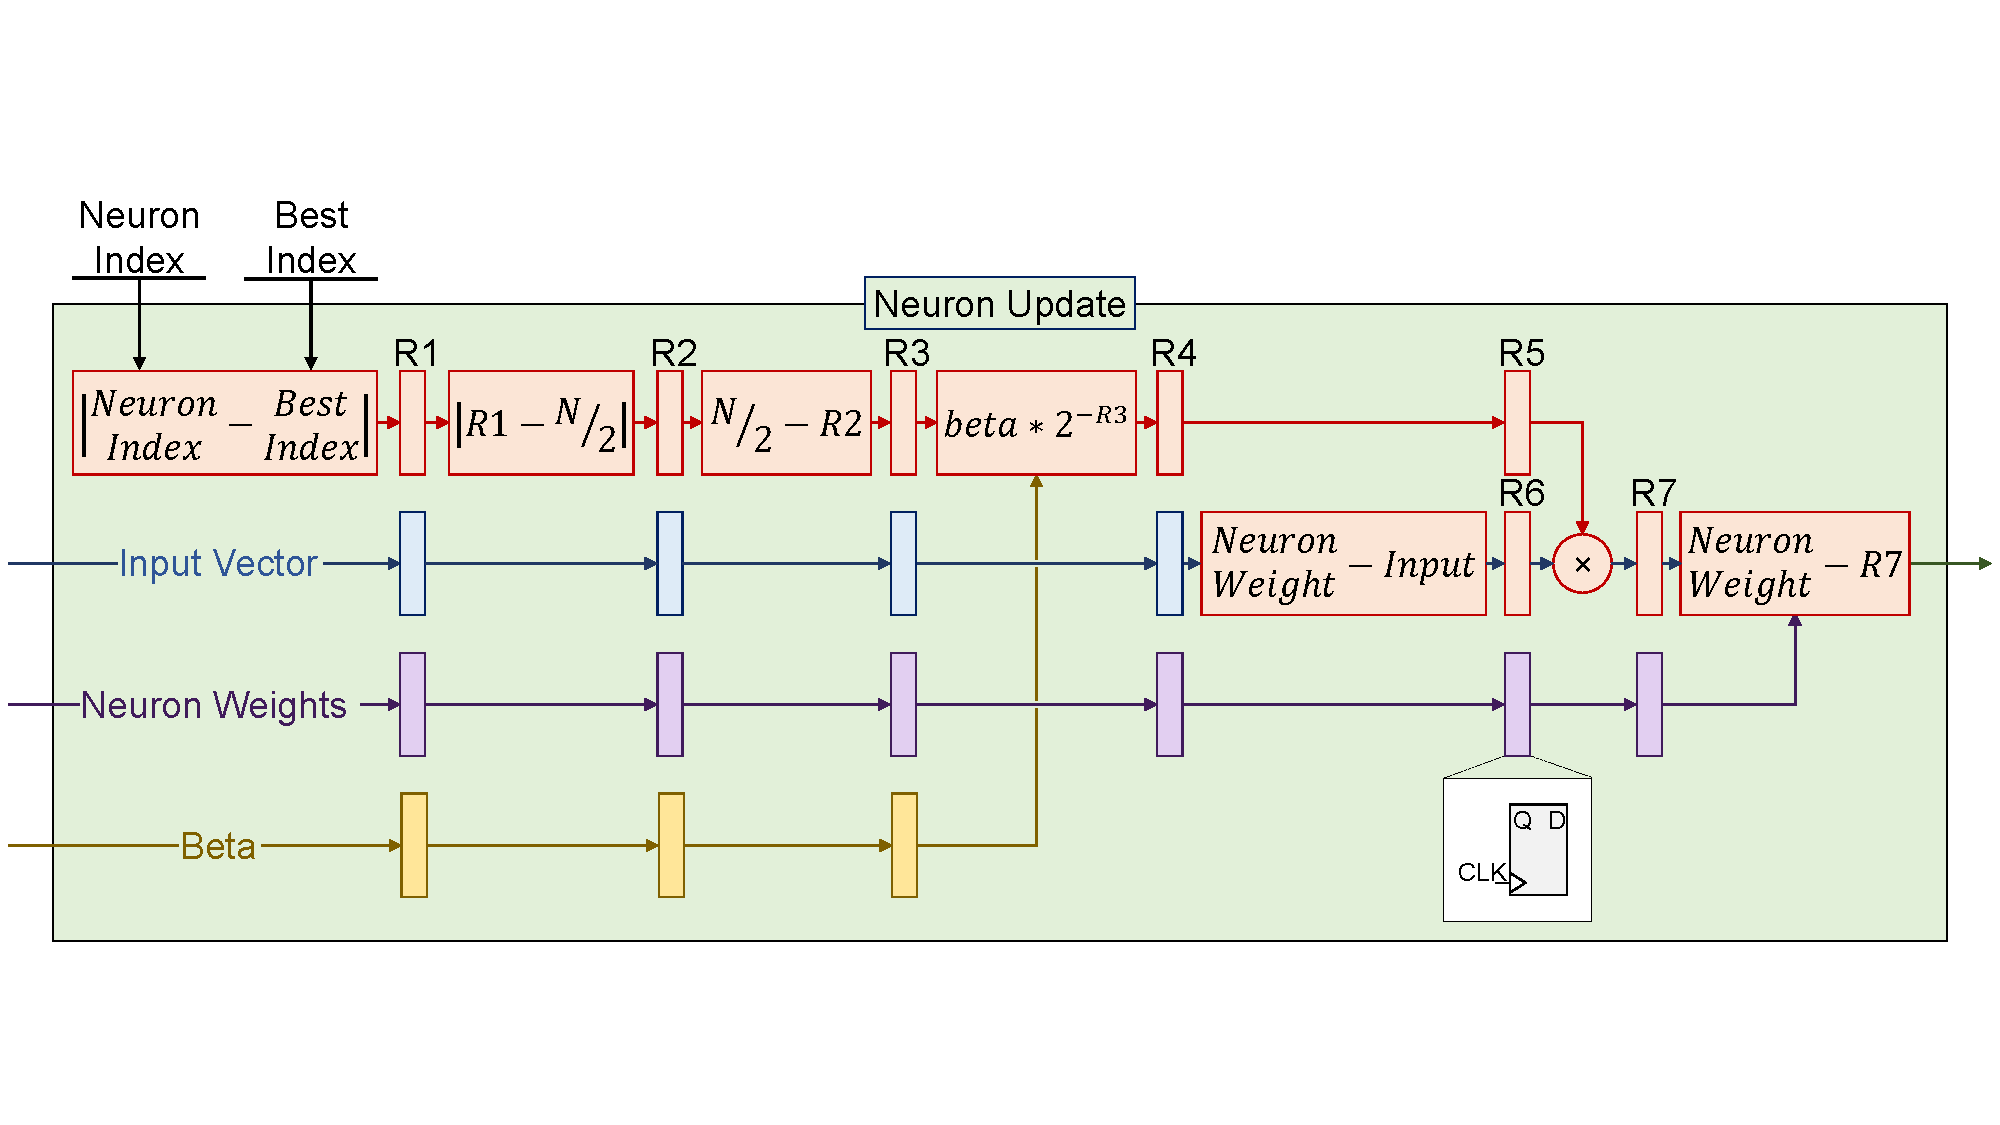
\includegraphics[width=0.48\textwidth]{./somResults/neuronUpdate_v2}
		\label{fig:NeuronUpdate}}
	\caption{(a) Hardware Module for BioSOM. (b) Neuron Update Module.}	\label{fig:SOMFPGAImplementation}
	\vspace{-1.0em}	
\end{figure}

During the training phase \textit{Neuron Update} component is enabled by setting (\textit{Update Enable=1}). The weights of the Neurons are updated using the distance output of the \textit{Compute Distance} module. The \textit{Neuron Update} component is also pipe-lined design with II=1. The pipeline stages are shown in Figure \ref{fig:NeuronUpdate}.
\subsection{Results}
The SOM has been implemented with a range of fixed-point formats. With fewer bits, one naturally expect that the SOM network for bacterial identification to suffer from accuracy degradation. A MATLAB simulation model was created to analyze the accuracy loss when using fixed-point implementation. We trained 10 SOMs with 10 different bacteria DNA sequences. Each SOM network has 100 neurons inside, and each neuron has 20 weights. We trained the networks by two independent training processes running in parallel. One is implemented using double precision floating point and the other is implemented with fixed-point weights. After training, we used the trained networks to identify the unknow sequence and record their scores.

The FPGA design is implemented with Vivado v.2016.4 used for synthesis and analysis of the HDL Designs. Our design is implemented in VHDL and validated using the Vivado simulator. Experimentation is done for different fixed point representations of weights by modifying parameters in VHDL code. 

\begin{figure*}[htb]
	\centering
		\subfloat[]{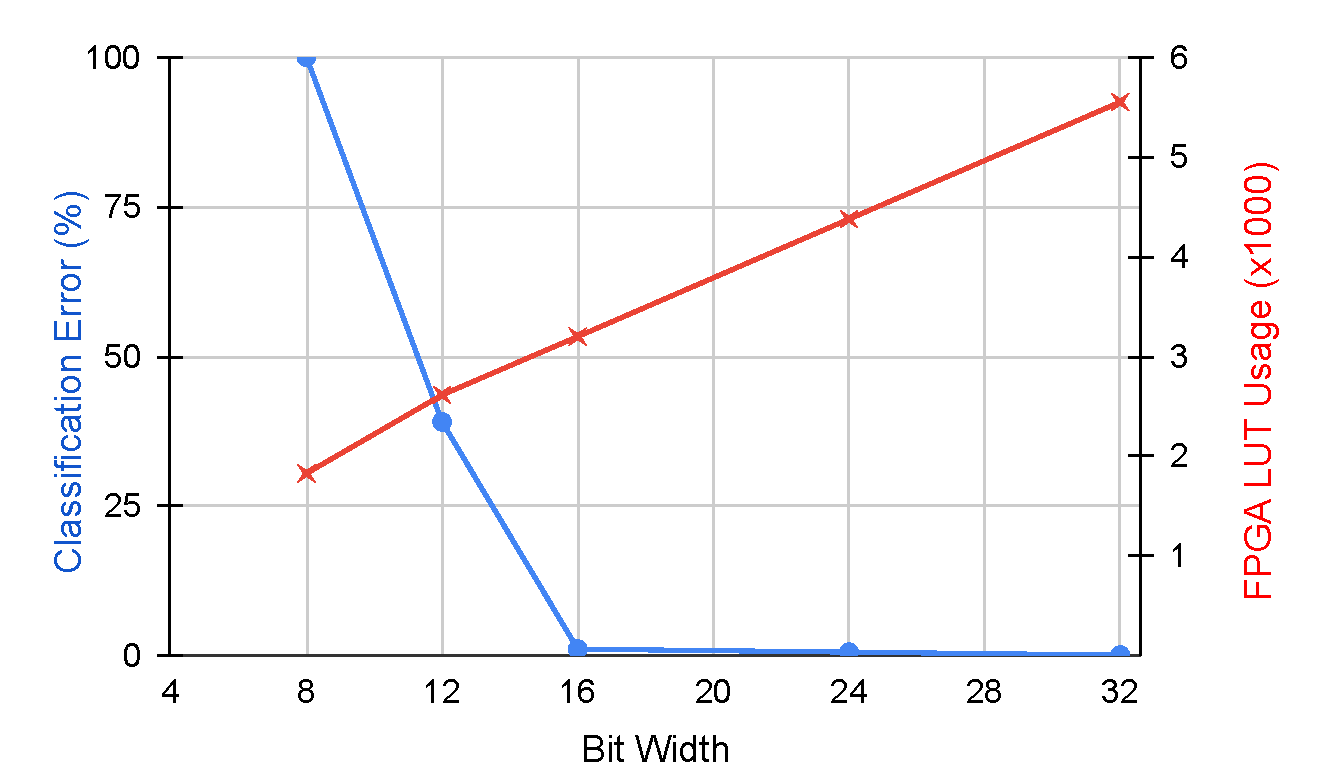
\includegraphics[width=0.45\textwidth]{./somResults/area}
		\label{fig:area}}
	\hfil
		\subfloat[]{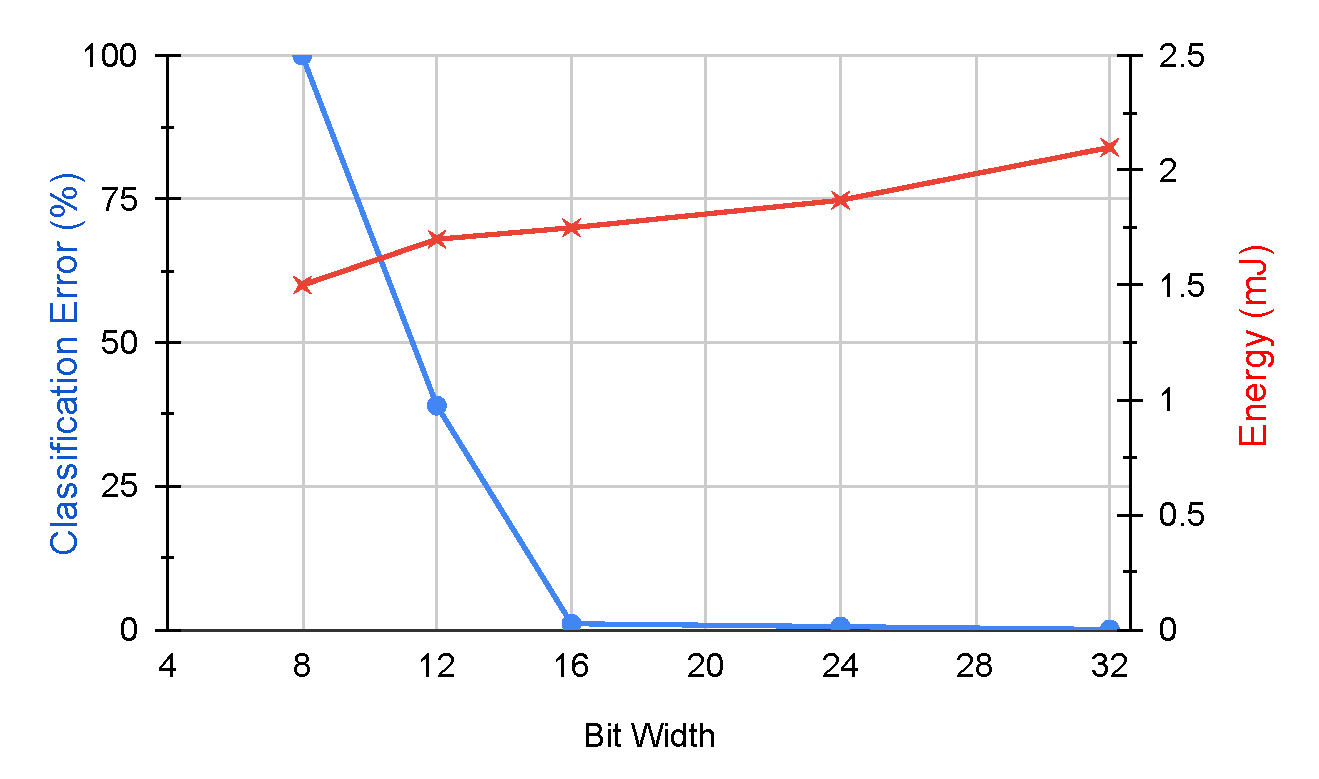
\includegraphics[width=0.45\textwidth]{./somResults/energy}
		\label{fig:energy}}
	\caption{comparison between different fixed-point fromat (a) FPGA LUT utilization (b) energy.}
	\label{fig:metrics}
\end{figure*}

The area and power numbers for different weight resolutions are extracted from the reports generated by Vivado tool post placement and routing with a working frequency of 100 MHz. Table \ref{table:1} compares the resources and area for 8, 12, 16, 24, and 32 bits fixed point formats, for a SOM network with 512 neurons. The second part of the table compares the average power in the different fixed point formats, for the same SOM.

The results are summarized in the Figure \ref{fig:area} and \ref{fig:energy}. Both the amount of utilized LUTs and total energy in Joule is presented against the classification error. From the figures, we can easily conclude that, we can substantially reduce the resources used and the energy by using a 16-bit fixed-point representation, without losing accuracy. We can reduce the resources even further by moving to the 12-bit representation, by sacrificing 39\% of the SOM accuracy. 
\begin{table}[h!]
	\centering
	\caption{Resource Comparison of different fixed point formats}
	\label{table:1}
	\begin{tabular}{ c |c | c| c |c | c } 
		\toprule
		Resource & 8b & 12b & 16b & 24b & 32b \\ 
		\midrule
		LUTs & 1823 & 2611 &3196 & 4375 & 5549 \\
		\hline
		Registers & 3481 & 4679 & 5871 & 8255 & 10639 \\ 
		\hline
		Slice & 854 & 1158 & 1369 &1809 & 2395 \\ 
		\hline
		LUT FF Pairs & 1007 & 1369 & 1750 & 2372 & 3043 \\
		\hline
		B-RAM & 4 & 6 & 8 & 11 & 15 \\
		\hline
		DSP48E1 & 17 & 17 & 17 & 17 & 33 \\
		\hline
		Bonded IOB & 57 & 61 & 65 & 73 & 81 \\
		\midrule
		%    \end{tabular}
	%\end{table}
	
	%\begin{table}[h!]
	%    \centering
	%    \caption{Power Comparison of different fixed-point formats}
	%    \label{table:2}
	%    \begin{tabular}[t]{ c |c | c| c |c | c } 
		\midrule
		Power(W) & 8b & 12b & 16b & 24b & 32b \\ 
		\midrule
		Total Power & 0.295 &0.314 &0.332 &0.356 &0.392 \\
		\hline
		Dynamic &0.052 &0.071 &0.089 &0.113 &0.148 \\ 
		\hline
		Device Static &0.243 &0.243 &0.243 &0.244 &0.244 \\ 
		\bottomrule
	\end{tabular}
\end{table}
\section{Conclusion}
With the sudden surge in Neural Network based applications, there is a pressing need for improving the performance and energy efficiency of DNN accelerators for their ubiquitous usage in energy constrained devices. The performance of DNN accelerator's is limited by the memory bandwidth and off-chip memory accessed dominates the energy consumption. The key to improving the energy efficiency of these NN is reducing the expensive off-chip memory accesses. Towards this we proposed approaches to reduce the off-chip memory accesses for DNNs. The proposed approaches optimizes the data reuse from on-chip memories for CNNs and LSTMs by partioning the data and scheduling the operations intelligently, without compromising the accuracy. We have also analyzed the impact of low bit resolution on the accuracy and energy, area performance. 
%\footnotesize
\bibliographystyle{abbrv} %IEEEtran % abbrv
%\vspace{1.5mm}
\bibliography{refs}
%\nocite{*}
%\end{spacing}

\end{document}
